\documentclass[UTF8]{ctexrep}

\usepackage{fancyhdr}
\usepackage[letterpaper, left=1in, right=1in, top=1in, bottom=1in]{geometry}
\usepackage{sectsty}
\usepackage{graphicx}
\usepackage{subfig}
\usepackage[section]{placeins}
\usepackage{hyperref}
\usepackage{amsmath}
\usepackage{listings}
\usepackage{color}
\usepackage{lstautogobble}

\definecolor{dkgreen}{rgb}{0,0.6,0}
\definecolor{gray}{rgb}{0.5,0.5,0.5}
\definecolor{mauve}{rgb}{0.58,0,0.82}

\lstset{frame=tb,
    language            = C,
    aboveskip           = 3mm,
    belowskip           = 5mm,
    showstringspaces    = false,
    columns             = flexible,
    basicstyle          = {\small\ttfamily},
    numbers             = none,
    numberstyle         = \tiny\color{gray},
    keywordstyle        = \color{blue},
    commentstyle        = \color{dkgreen},
    stringstyle         = \color{mauve},
    breaklines          = true,
    breakatwhitespace   = true,
    tabsize             = 3,
    % numbers             = left,
    % numberblanklines    = true,
    firstnumber         = 1,
    numberstyle         = \scriptsize\color{black},
    numbersep           = 12pt,
    mathescape          = true
    % autogobble          = true
}

\usepackage{xcolor}

\definecolor{codegreen}{rgb}{0,0.6,0}
\definecolor{codegray}{rgb}{0.5,0.5,0.5}
\definecolor{codepurple}{rgb}{0.58,0,0.82}
\definecolor{backcolour}{rgb}{0.95,0.95,0.92}

\lstdefinestyle{mystyle}{
    backgroundcolor=\color{backcolour},
    commentstyle=\color{codegreen},
    keywordstyle=\color{magenta},
    % numberstyle=\tiny\color{codegray},
    stringstyle=\color{codepurple},
    basicstyle=\ttfamily\footnotesize,
    breaklines=true,
    captionpos=b,
    keepspaces=true,
    showspaces=false,
    showstringspaces=false,
    showtabs=false,
    tabsize=4
}

\lstset{style=mystyle}
\let\origthelstnumber\thelstnumber
\makeatletter
\newcommand*\Suppressnumber{%
  \lst@AddToHook{OnNewLine}{%
    \let\thelstnumber\relax%
     \advance\c@lstnumber-\@ne\relax%
    }%
}

\newcommand*\Reactivatenumber[1]{%
  \setcounter{lstnumber}{\numexpr#1-1\relax}
  \lst@AddToHook{OnNewLine}{%
   \let\thelstnumber\origthelstnumber%
   \refstepcounter{lstnumber}
  }%
}


\makeatother
\hypersetup{
    colorlinks=true,
    linkcolor=blue,
    filecolor=magenta,
    urlcolor=blue,
}
\allsectionsfont{\mdseries\scshape}

\renewcommand{\thesection}{\arabic{section}}

\newcommand{\horrule}[1]{\rule{\linewidth}{#1}}
\title{
    \horrule{0.5pt} \\[0.4cm]
    \huge Final Project \\
    \horrule{2pt}
}
\author{
    陈思贝 (718030290013)
}
\date{
    % TODO: Date
}
\setcounter{section}{-1}

\begin{document}
    \maketitle

    \section{实验配置}

    \begin{itemize}
        \item Linux Kernel: 5.4.126
        \item OS: Ubuntu 18.04.5 LTS
        \item Architecture: x86\_64
    \end{itemize}
    \vspace{.3cm}

    \section{实验过程}

    本次实验修改系统调用表(\texttt{sys\_call\_table})中的\texttt{\_\_NR\_clone}系统调用。其中难点主要分为3个部分,定位系统调用表、修改内存权限为可读以及对系统调用表进行替换。\\

    \subsection{定位系统调用表}

    在x86系统中可以使用\texttt{linux/kallsysms.h}中定义的\texttt{kallsyms\_lookup\_name("sys\_call\_table")}直接找出系统调用表的内存位置。

    \begin{lstlisting}
        static unsigned long *syscall_table;

        syscall_table = (void *) kallsyms_lookup_name("sys_call_table");
        if (!syscall_table) {
            printk(KERN_ERR "Syscall_table not found");
            return -1;
        }\end{lstlisting}

    系统调用表中通过\texttt{\_\_NR\_clone}访问原先的系统调用处理函数。为事后复原系统调用表,这里用一个自定义指针储存一下。
    \begin{lstlisting}
        typedef long(sys_clone) (unsigned long, unsigned long, int __user *, int __user *, unsigned long);
        static sys_clone *old_clone;
        
        old_clone = (sys_clone *)syscall_table[__NR_clone];\end{lstlisting}

    \subsection{修改内存权限}

    系统调用表所在内存是只读内存,因此我们需要将该块内存改为可读写内存。除此之外,x86系统还对该块区域内存做出了保护,需要对\texttt{WP flag}进行修改。这个flag用于阻止CPU写入只读内存页。

    \begin{lstlisting}
        inline void mywrite_cr0(unsigned long cr0) {
            asm volatile("mov %0,%%cr0" : "+r"(cr0));
        }

        #define unprotect_memory() \
        ({ \
            orig_cr0 =  read_cr0();\
            mywrite_cr0(orig_cr0 & (~ 0x10000)); /* Set WP flag to 0 */ \
        });
        #define protect_memory() \
        ({ \
            mywrite_cr0(orig_cr0); /* Set WP flag to 1 */ \
        });\end{lstlisting}

    \subsection{替换系统调用表}
    在修改过内存权限后,就可以对系统调用表进行替换了。首先调用在第一部中存着的原来的系统调用,然后向内核输出替换掉用成功的信息,并返回原来调用的返回值。
    
    \begin{lstlisting}
        asmlinkage long sys_clone_hook(unsigned long x1, unsigned long x2, int __user *x3, int __user *x4, unsigned long x5) {
            long ret_val = old_clone(x1, x2, x3, x4, x5);
            printk(KERN_INFO "hello, I have hacked this syscall");
            return ret_val;
        }
        unprotect_memory();
        syscall_table[__NR_clone] = (unsigned long)sys_clone_hook;
        protect_memory();\end{lstlisting}

    在退出模块的时候,将系统调用表恢复成原来的程序即可。

    \begin{lstlisting}
        unprotect_memory();
        syscall_table[__NR_clone] = (unsigned long)old_clone;
        protect_memory();\end{lstlisting}

    \section{实验效果截图}

    \begin{enumerate}
        \item 第一次测试(图\ref{ref:demo1})仅运行\texttt{dmesg}指令,新增1条输出(\texttt{dmesg})。
        \begin{figure}[h!]
            \centering
            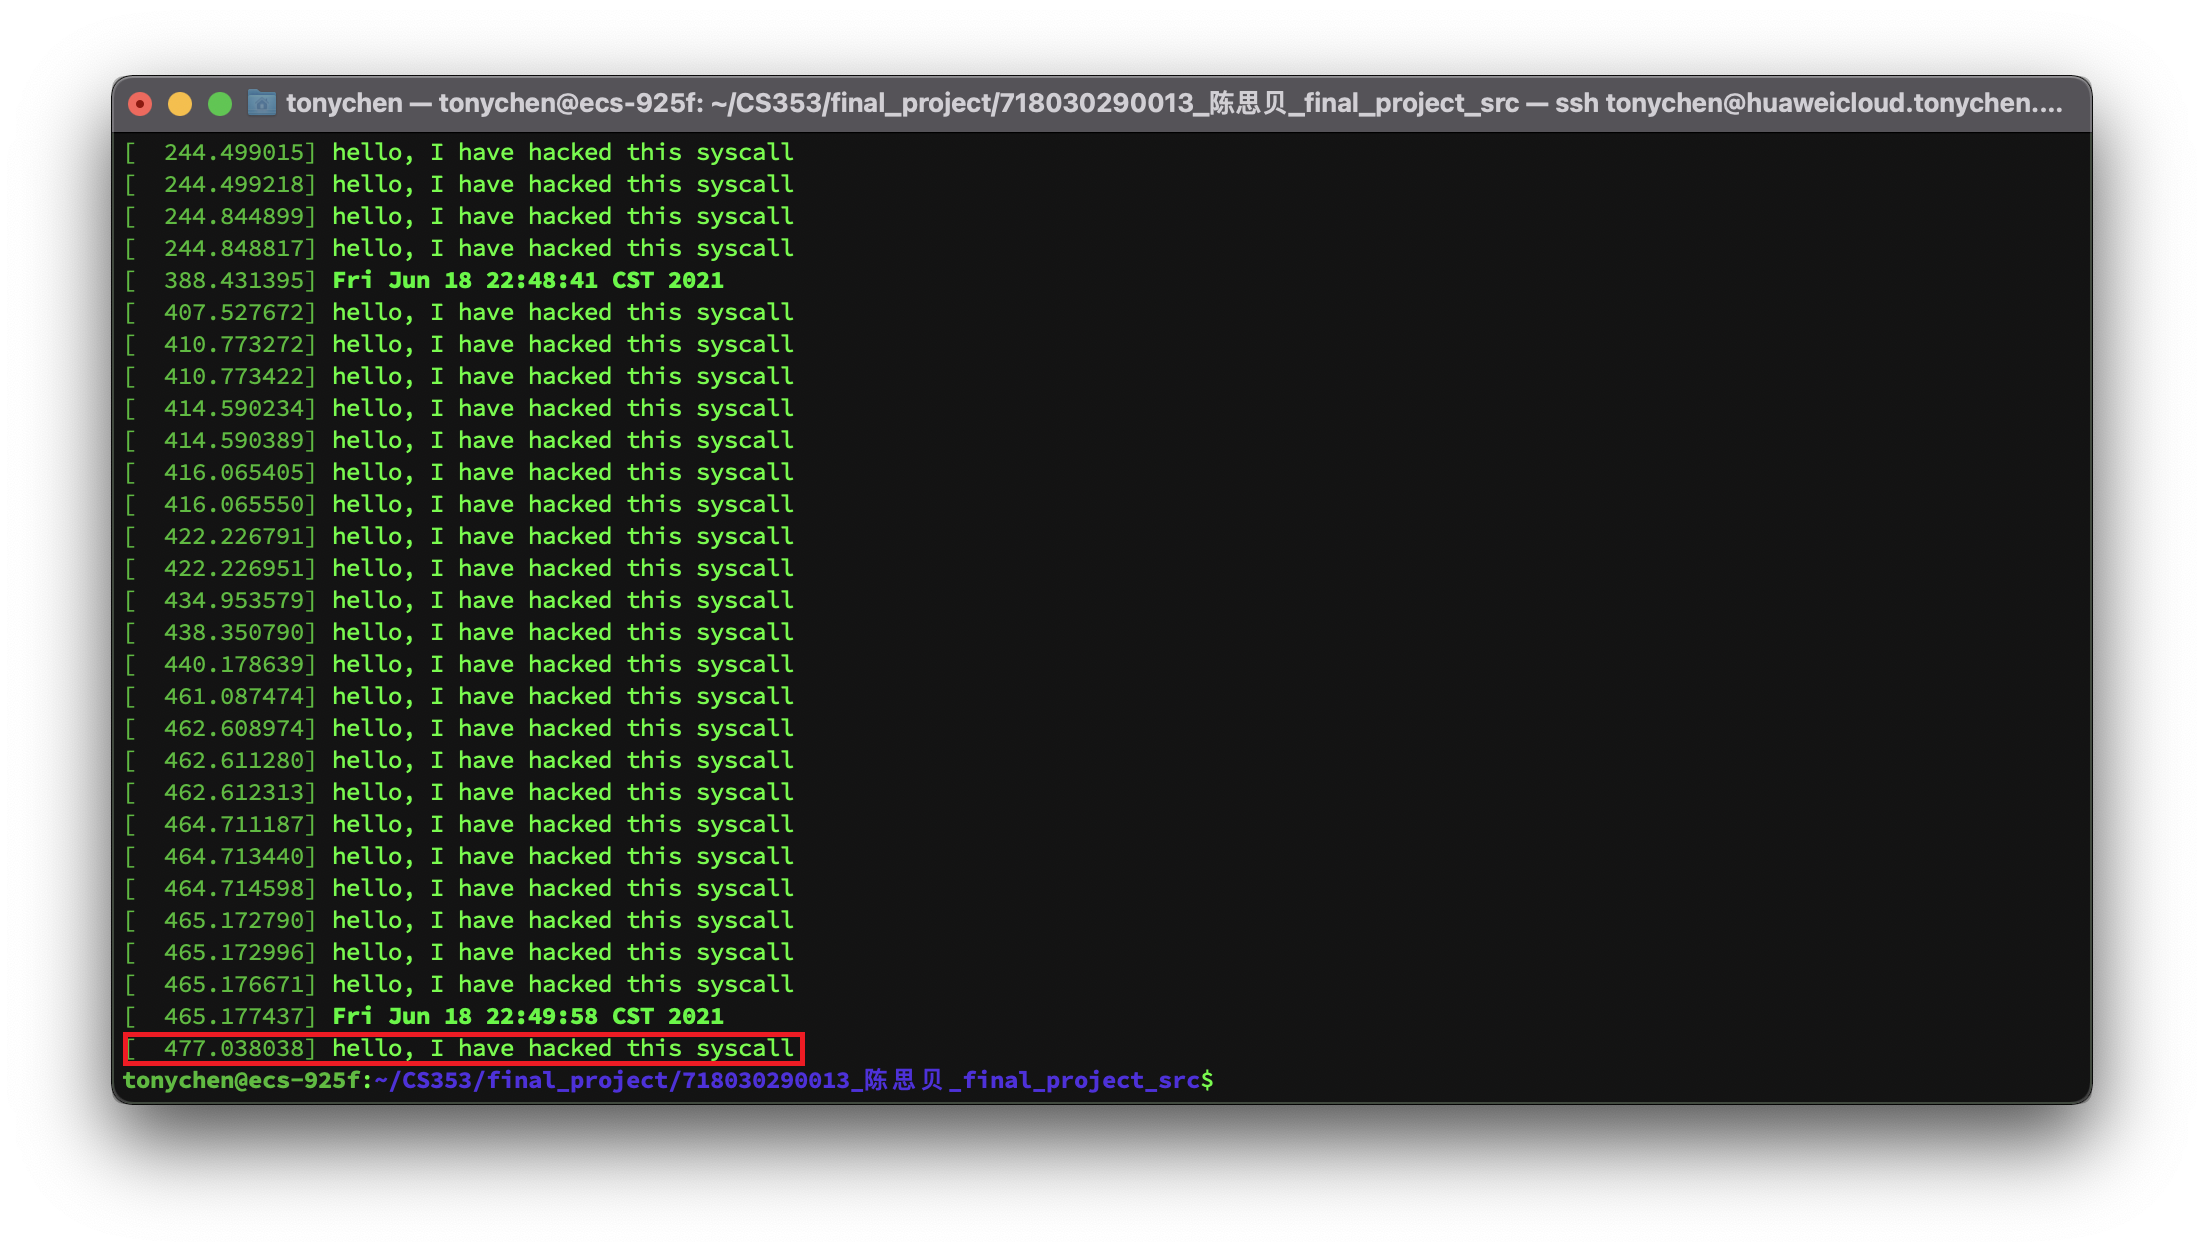
\includegraphics[width=15cm,keepaspectratio]{images/demo1.png}
            \caption{第一次测试}
            \label{ref:demo1}
        \end{figure}
        \clearpage
        \item 第二次测试(图\ref{ref:demo2})运行\texttt{test.o}后通过\texttt{dmesg}查看,新增2条输出(\texttt{test.o} * 1 和 \texttt{dmesg} * 1)。
        \begin{figure}[h!]
            \centering
            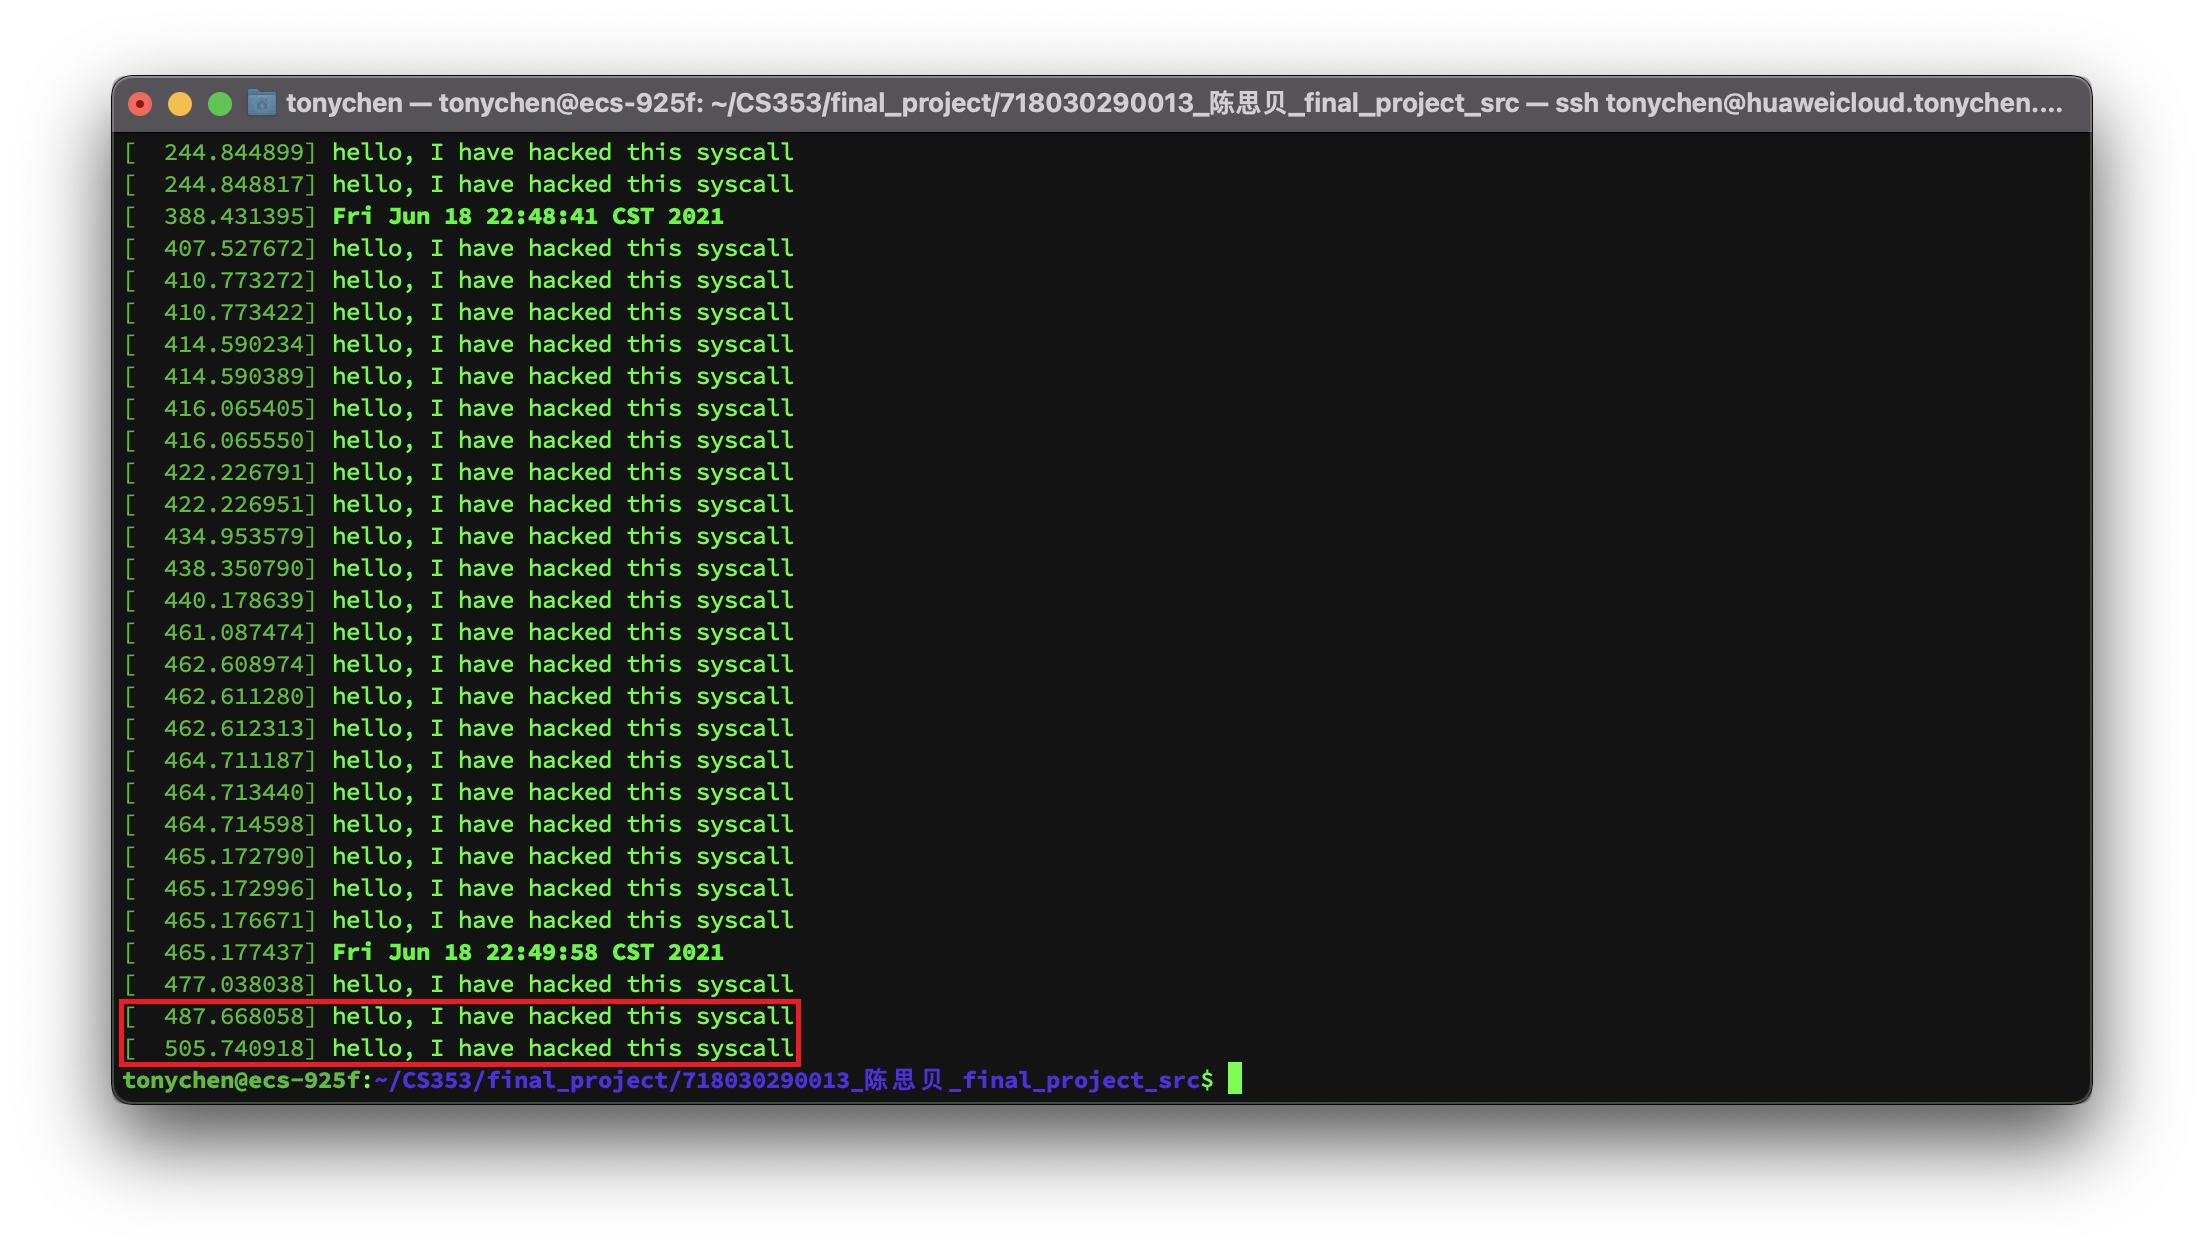
\includegraphics[width=15cm,keepaspectratio]{images/demo2.png}
            \caption{第二次测试}
            \label{ref:demo2}
        \end{figure}
        \item 第三次测试(图\ref{ref:demo3})运行\texttt{bench.o}后通过\texttt{dmesg}查看,新增7条输出(\texttt{bench.o} * 6 和 \texttt{dmesg} * 1)。
        \begin{figure}[h!]
            \centering
            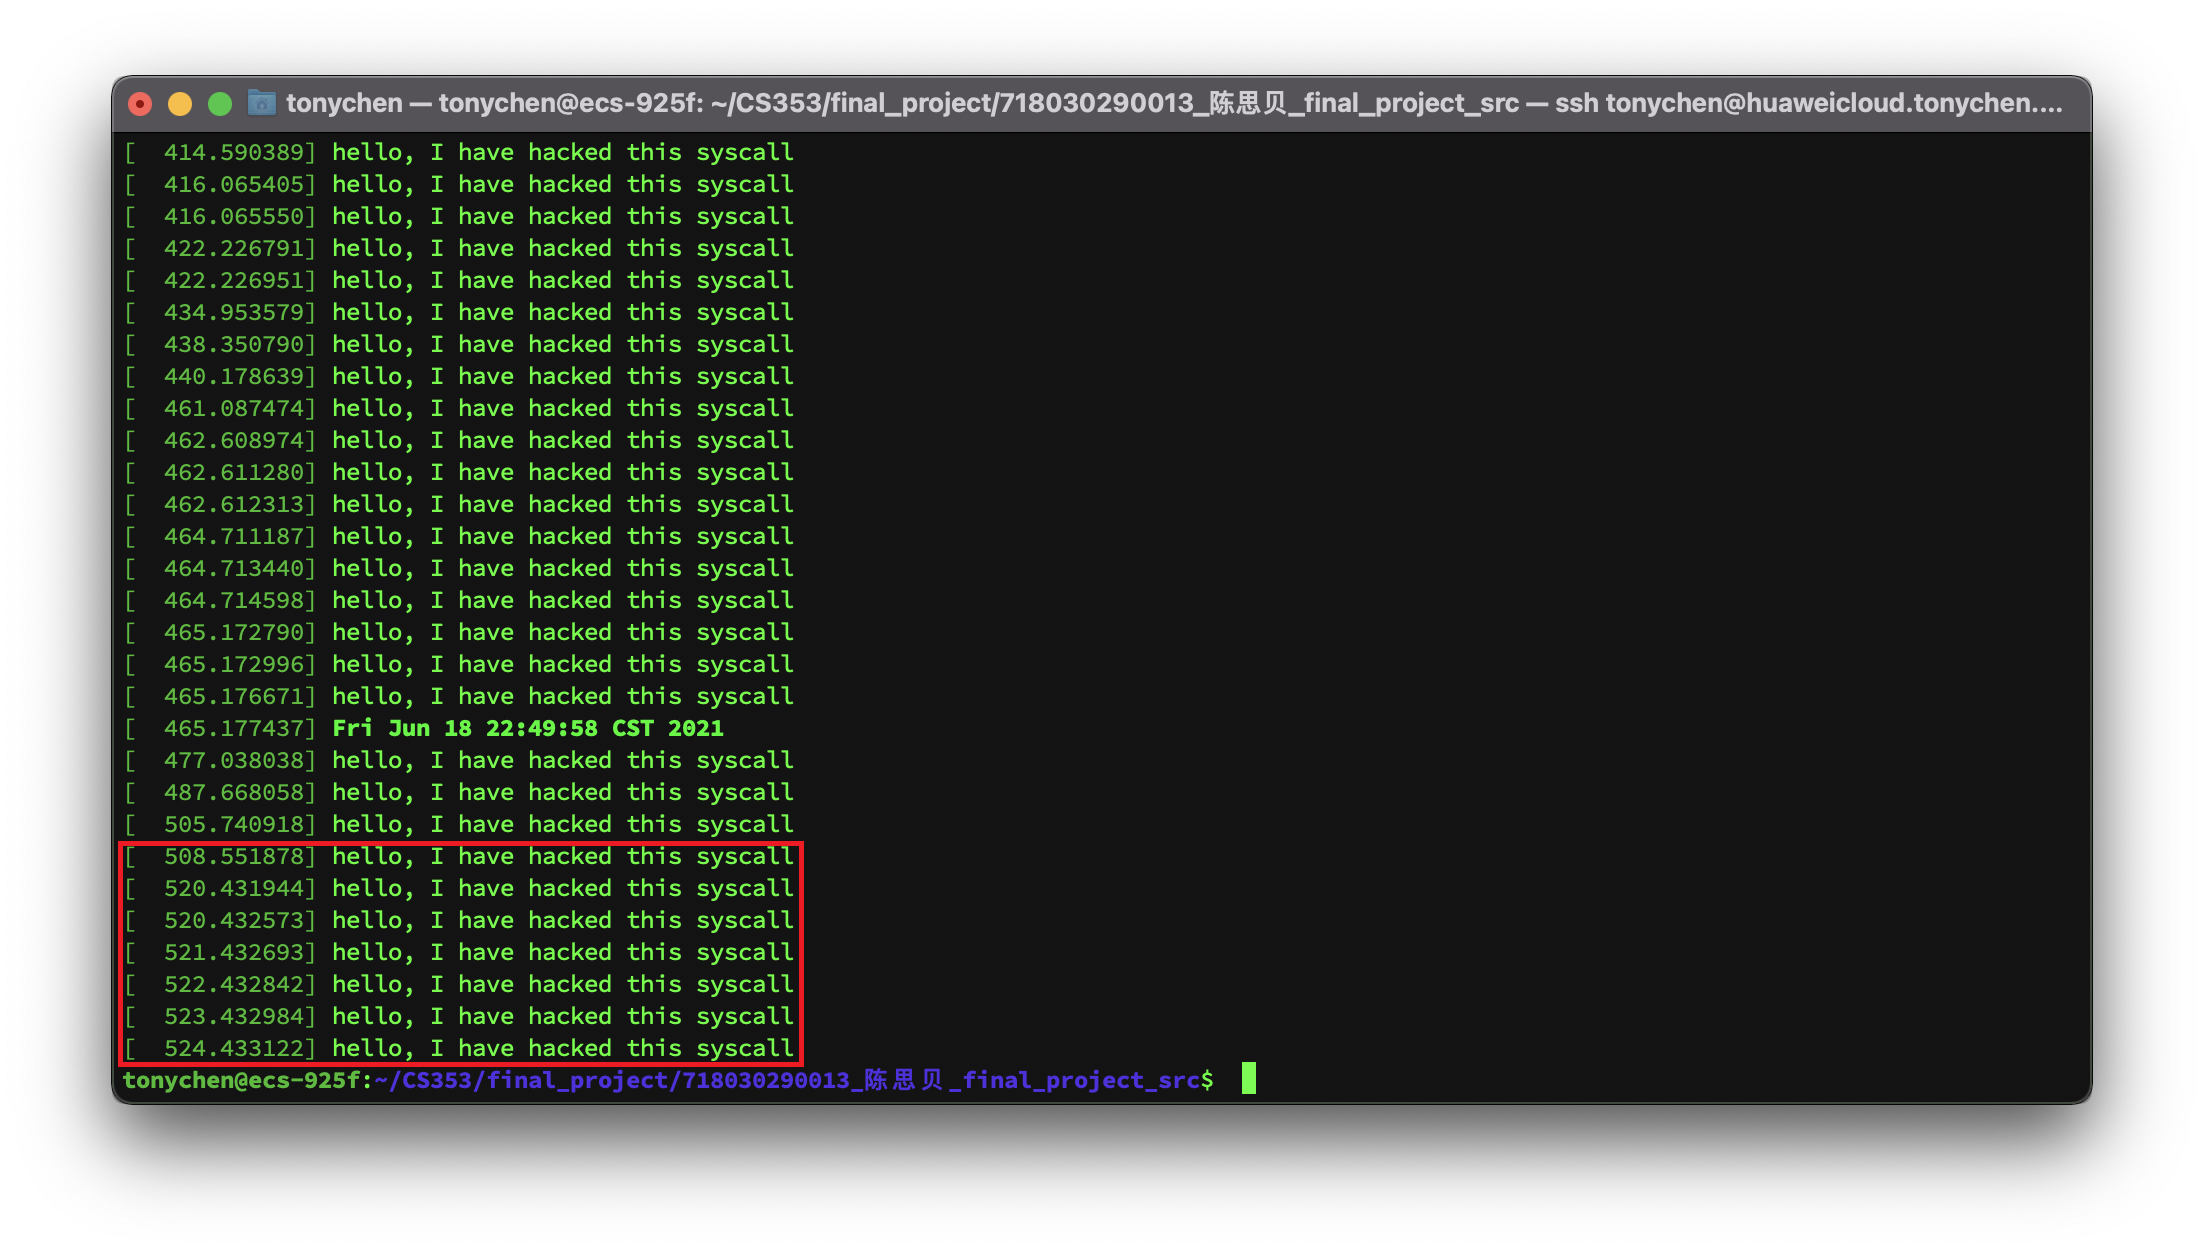
\includegraphics[width=15cm,keepaspectratio]{images/demo3.png}
            \caption{第三次测试}
            \label{ref:demo3}
        \end{figure}
    \end{enumerate}

    \section{实验心得}

    通过本次的实验,对Linux中系统调用表有了更深的理解。对于该文件和其他辅助头文件的阅读,对系统调用操作有了更深的理解。通过对网上公开的代码示例的分析,成功完成了这次实验。\\
    
    \section{参考资料}
    
    \begin{enumerate}
        \item \href{https://stackoverflow.com/questions/58512430/how-to-write-to-protected-pages-in-the-linux-kernel/60564037#60564037}{How to write to protected pages in the Linux kernel? - StackOverflow}
        \item \href{https://infosecwriteups.com/linux-kernel-module-rootkit-syscall-table-hijacking-8f1bc0bd099c}{Linux Kernel Module Rootkit — Syscall Table Hijacking}
        \item \href{https://stackoverflow.com/questions/2103315/linux-kernel-system-call-hooking-example}{Linux Kernel: System call hooking example - StackOverflow}
        \item \href{https://www.kernel.org/doc/html/latest/process/adding-syscalls.html}{Adding a New System Call}
    \end{enumerate}
    \vspace{.3cm}

\end{document}